\chapter{Polymorphism}
Polymorphism basically means \textit{``many forms''}, where \textit{forms} are \textbf{types}.
Thus there may be \textit{polymorphic} function names, or \textit{polymorphic} types.

\begin{paracol}{2}
    
    There are many ``flavors'' of polymorphism, many variations.
    Two main kinds opposed to each other are \textit{ad hoc} and \textit{universal} polymorphism, which however, may coexist:
    \begin{itemize}
        \item \textbf{ad hoc} PM indicates that a single function name denotes different algorithms, determined by the actual types.
        \item \textbf{universal} PM indicates a single algorithm (solution) applicable to objects of different types.
    \end{itemize}

    In example \ref{lst:polymorphism_coexist} we can see how the two kinds of polymorphism can coexist in the same code:
    \lstinline|setValue(T v1)| uses the same algorithm, but applied to object of different types \textit{universal}, but at the same time, provides ad hoc polymorphism due to ``overloading'', i.e. the same function name applied to different types, denoting different algorithms.

    \switchcolumn

    \begin{lstlisting}[label={lst:polymorphism_coexist},caption={Coexistence of ad hoc and universal polymorphism},captionpos=b]
class Box<T,V> {
    private T v1;
    private V v2;

    public void setValue(T v1) {
        this.v1 = v1;
        ...
    }
    public void setValue(V v2) {
        this.v2 = v2;
        ...
    }
    public void setValue() {
        this.v1 = null;
        this.v2 = null;
    }
}
    \end{lstlisting}
\end{paracol}


When PM is taken into account, it is crucial to consider when happens the \textbf{binding} between a function name and the actual code to be executed:
\begin{itemize}
    \item compile time; \textit{static/early binding}
    \item linking time
    \item execution time; \textit{late/dynamic binding}
\end{itemize}
In general the earlier the binding happens, the better (for debugging reasons).
If the binding spans over more phases (e.g. \textit{overriding} in Java), as a convention we consider the \textbf{binding time} the last phase.

\begin{figure}[h]
    \centering
    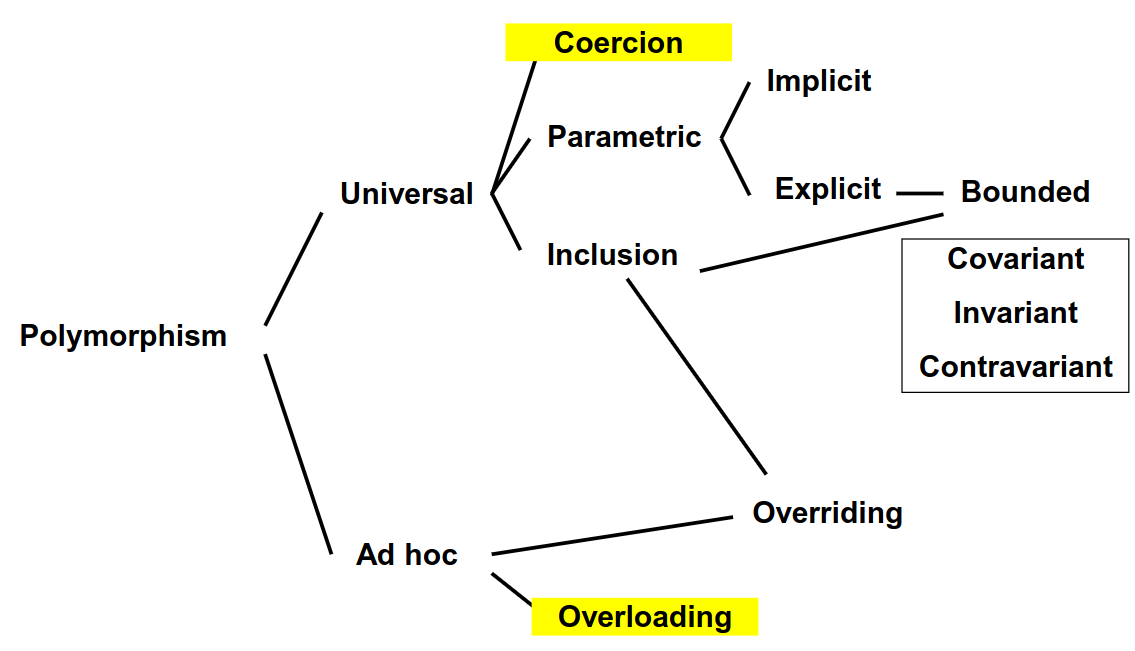
\includegraphics[width=0.7\textwidth]{images/polymorphism.png}
    \caption{Polymorphism classification}
    \label{fig:polymorphism_classification}
\end{figure}
\section{Overloading - Same name, different types}
\textbf{Overloading} is present in every language for basic operators $+-*...$,
and sometimes is supported for user-defined functions, 
and in some languages it is even allowed the overloading of primitive operator by user-defined functions.\\
Since this falls under the \textbf{ad hoc} polymorphism family,
the code to be executed is determined by the type of the arguments;
the binding can either happen at \textit{compile} or at \textit{runtime},
depending on the typing of the language,
whether it is static or dynamic.

\begin{lstlisting}
    // C language doesn't allow overloading for user-defined functions
    int sqrInt(int x) { return x * x; }
    double sqrDouble(double x) { return x * x; }
    
    // Overloading in Java & C++
    int sqr(int x) { return x * x; }
    double sqr(double x) { return x * x; }
\end{lstlisting}

\subsection{Haskell and Rust}
\lstset{language=Haskell, basicstyle=\footnotesize\ttfamily}
\begin{paracol}{2}

    Haskell introduces \textbf{type classes} for handling
    overloading in presence of type inference.\\
    A type class defines a set of functions that can be implemented by different types. For example, the \lstinline|Eq| type class defines the equality operator (\lstinline|==|) which can be used to compare integers, characters, and other types.
    
    Haskell's compiler can automatically determine the types of expressions without explicit type annotations. Type classes work seamlessly with \textbf{type inference} to ensure that the correct function implementation is chosen based on the inferred types.
    \switchcolumn
    
    
    \begin{lstlisting}
        -- Define a custom data type
        data Color = Red | Green | Blue
        
        -- Make Color an instance of Eq
        instance Eq Color where
        Red == Red = True
        Green == Green = True
        Blue == Blue = True
        _ == _ = False
        
        -- Example usage
        main :: IO ()
        main = do
        print (Red == Red)   -- Output: True
        print (Red == Green) -- Output: False
    \end{lstlisting}
\end{paracol}
    

\lstset{language=Rust}
In Rust instead has \textbf{Traits} which are similar to type classes in Haskell: they define a set of methods that a type must implement.

\begin{lstlisting}
use std::ops::Add;
// Define a custom struct
#[derive(Debug)]
struct Point {
    x: i32,
    y: i32,
}

// Implement the Add trait for Point
impl Add for Point {
    type Output = Point;

    fn add(self, other: Point) -> Point {
        Point {
            x: self.x + other.x,
            y: self.y + other.y,
        }
    }
}
\end{lstlisting}

\lstset{style=javaBlockAnn}
\section{Coercion - Implicit conversion}
\textbf{Coercion} is the automatic (implicit) conversion of an object to a different type, opposed to casting which is explicit instead.
Coercion allows a code snippet to be applied of arguments of different (convertible) types.
Sometimes coercion is allowed only if there is no \textbf{information loss}.

\begin{lstlisting}
    double sqrt(double x){...}
    double d = sqrt(5) // applied to int
\end{lstlisting}

\subsection{Java}
Java allows coercion between primitive types, but not between primitive types and objects.
However, among ---some--- objects, Java \textbf{autoboxing} and unboxing is allowed, which is automatic conversion between primitive types and their corresponding wrapper classes.
\begin{lstlisting}
    Integer i = 5; // autoboxing
    int j = i;     // unboxing
\end{lstlisting}

In Java there is also \textbf{upcasting} and \textbf{downcasting}, which allow coercion between superclass and subclass types.
\begin{lstlisting}
Dog dog = new Dog();
Animal animal = dog; // Upcasting
...
Animal animal = new Dog();
Dog dog = (Dog) animal; // Downcasting
\end{lstlisting}

\begin{lstlisting}[caption={Other examples of coercion in Java},captionpos=t]
    int num = 10;
    if (num) { // num is implicitly converted to boolean
    ...

    double d = 9.78;
    int i = (int) d; // Explicit casting from double to int

    int num = 100;
    String str = "Number: " + num; // int to String
\end{lstlisting}

\section{Inclusion Polymorphism - Inheritance}
Inclusion polymorphism is also known as \textit{subtyping polymorphism} or \textit{\textbf{inheritance}}.
It is ensured by \textit{Barbara Liskov}'s \textbf{substitution principle}:
\begin{definition}[Liskov Substitution Principle]
    \textit{A subtype object can be used in any context where a supertype object is expected}
\end{definition}
Methods and fields defined in a superclass may be invoked and accessed by subclasses if not redefined (see \textit{Overriding}).\\
Note, again, that this refers to \ul{using superclass methods, not overriding them.}\\
Override would possibly break the substitution principle, because the subclass method may have a different behavior than the superclass method.

\section{Overriding - Same name, same types, but in subclasses}
In Java a method $m$ of a
class $A$ can be redefined
in a subclass $B$ of $A$.

Overriding introduces ad hoc polymorphism in the universal polymorphism of inheritance.
Notice that even though written in the subclass definition, overriding requires the final binding to happen at runtime:
it happens through the lookup done by \lstinline{invokevirtual} in the JVM.

\section{C++ vs Java}
\begin{lstlisting}[language=C++]
class A {
 public:
  virtual void onFoo() {}
  virtual void onFoo(int i) {}
};
class B : public A {
 public:
  virtual void onFoo(int i) {}
};
class C : public B {};
int main() {
  C* c = new C();
  c->onFoo();
  // Compile error - doesn't exist
}
\end{lstlisting}
The equivalent code in Java compiles, because in java invokes the function \lstinline{onFoo()} with no arguments defined in the superclass A.
In C++ instead, the function \lstinline|onFoo(int i)| defined in B is found and stops the search, but there is arguments type mismatch, thus it doesn't compile.
This happens because in C++ the method lookup is based on the method \textit{name}, not on its \textit{signature}.

The solution is to add using \lstinline|A::onFoo;| to class B.

\section{Parametric Polymorphism}
\subsection{Templates vs Generics}
\lstset{language=C++}

\textbf{Templates} are similar to \textit{Generics} in Java, 
they are used as function and class templates
each concrete instantiation produces a copy of the generic code, specialized for that type:
\textbf{monomorphization}.
In java Generics, instead, \textbf{type erasure} happens at runtime, i.e. type variables \lstinline{T} are replaced by \lstinline{Object} variables.\\
Templates support parametric polymorphism and\ul{ type parameters can also be primitive types (unlike Java generics)}
\begin{lstlisting}
    template <class T> // or <typename T>
    T sqr(T x) { return x * x; }
\end{lstlisting}
Assuming to invoke \lstinline{sqr(T x)} on variables of different types, the compiler will generate a specific code for each type used.
This works even on user-defined types;
check the following code for an example:
\begin{lstlisting}
class Complex {
 public:
  double real;
  double imag;
  Complex(double r, double im) : real(r), imag(im){};
  Complex operator*(Complex y) {  // overloading of *
    return Complex(real * y.real - imag * y.imag,
                   real * y.imag + imag * y.real);
  }
};

Complex cc = sqr(c); // legal and produces a function "Complex sqr(Complex x) {...}"
\end{lstlisting}

It is important to check for type ambiguosity;
in the following example, it is highlighted a case where it's not clear whether it is \lstinline{i} to be converted to \lstinline{long} or \lstinline{m} to \lstinline{i}.
\begin{lstlisting}
template <class T>
T GetMax(T a, T b) {  return (a > b) ? a : b; }
...
n = GetMax(l, m);       // ok: GetMax<long>
// v = GetMax(i, m);    // no: ambiguous
v = GetMax<int>(i, m);  // ok
\end{lstlisting}

\subsection{Macros}
\textbf{Macros} can be exploited to achieve \textit{polymorphism} and can have the same effect of the templates,
but notice that macros are executed by the preprocessor\footnote{Macro expansion can be seen using the option \textit{-E} when compiling} and are only \textbf{textual substition},
there is no parsing, no static analysis checks or whatsoever.
\note{But which type of polymorphism is this? }
\begin{lstlisting}
#define sqr(x) ((x) * (x))
int a = 2;
int aa = sqr(a++); // int aa = ((a++) * (a++));
// value of aa? aa contains 6  :(

#define fact(n) (n == 0) ? 1 : fact(n-1) * n
// compilation fails because fact is not defined
\end{lstlisting}

% \section*{16 - Ottobre}

\subsection{Specialization}
A template can be \textbf{specialized} by defining a template with the same name but with more specific parameters (\textit{partial specialization}) or with no parameters (\textit{full specialization}).
This is kinda similar to \textit{Overriding},
leaving to the compiler the choice of the most appropriate template.

\begin{lstlisting}
/* Primary template */
template <typename T> class Set {
        // Use a binary tree
    };
/* Full specialization */
template <> class Set<char> {
        // Use a bit vector
    };
/* Partial specialization */
template <typename T> class Set<T*> {
        // Use a hash table
    };
\end{lstlisting}

Templates can be used by a compiler to
generate temporary source code, which is
merged by the compiler with the rest of the
source code and then compiled.

Template compilation happens \textit{on demand}: the code of a template
is not compiled until an instantiation is required,
however in case of \textit{fully-specialized} template,
the compiler treats the template as a function, thus it generates its code \textbf{regardless} whether it is ever used or not.

Note that in C/C++ while method \textit{prototypes} usually are in a separate \lstinline{.h} file,
the compiler needs the template \textit{declaration} and \textit{definition} in the same place to instatiate it. 

\lstset{style=javaBlockAnn}